\documentclass{standalone}
\usepackage{tikz}
\usetikzlibrary{arrows}

\begin{document}
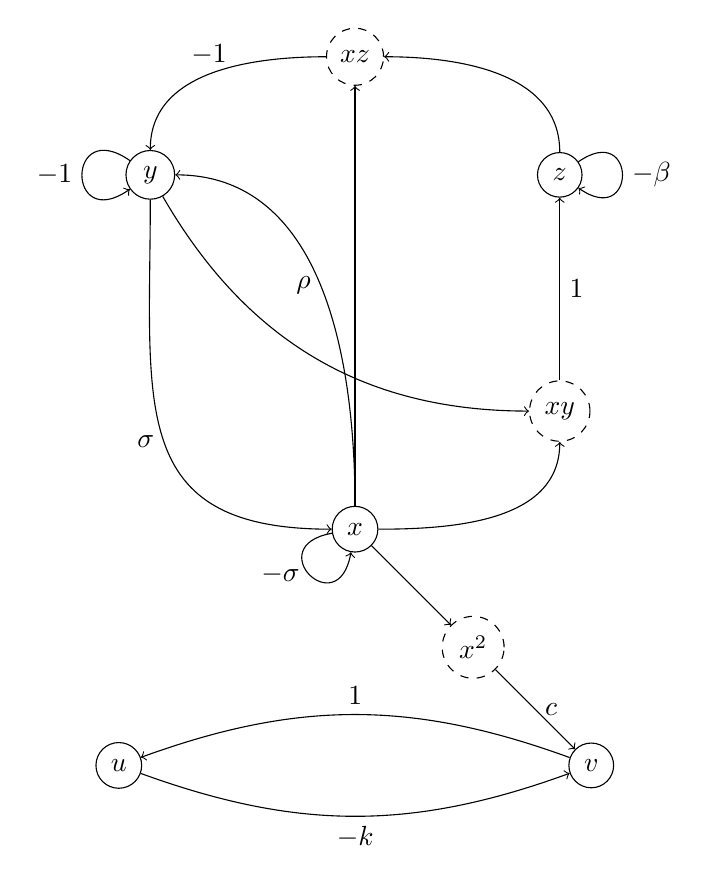
\begin{tikzpicture}
	\node[draw, circle, name=z] at (2.60, 1.5) {$z$};
	\node[draw, circle, name=y] at (-2.60, 1.5) {$y$};
	\node[draw, circle, name=x] at (0, -3) {$x$};
	\node[draw, circle, dashed, name=xz] at (0, 3) {$xz$};
	\node[draw, circle, dashed, name=xy] at (2.6, -1.5) {$xy$};
	\draw[->, out=270, in=180, looseness = 1.4] (y) to node[midway, left] {$\sigma$} (x);
	\draw[->, out=90, in=0] (z) to (xz);
	\draw[->, out=90, in=270] (x) to (xz);
	\draw[->, out=180, in=90] (xz) to  node[midway, above] {$-1$}(y);
	\draw[->, out=90, in=0] (x) to node[midway, left] {$\rho$} (y);
	\draw[->, out=0, in=270] (x) to (xy);
	\draw[->, out=300, in=180] (y) to (xy);
	\draw[->, out=90, in=270] (xy) to node[midway, right] {$1$}(z);
	\draw[->, out=190, in=260, looseness=7] (x) to node[midway, left] {$-\sigma$} (x) ;
	\draw[->, out=145, in=215, looseness=7] (y) to node[midway, left] {$-1$} (y) ;
	\draw[->, out=35, in=325, looseness=7] (z) to node[midway, right] {$-\beta$} (z) ;
	\node[draw, circle, name=v] at (3, -6) {$v$};
	\node[draw, circle, name=u] at (-3, -6) {$u$};
	\node[draw, circle, dashed, name=x2] at (1.5, -4.5) {$x^2$};
	\draw[->] (x) to (x2);
	\draw[->] (x2) -- (v) node[midway,right] {$c$};
	\draw[->, out=160, in=20] (v) to node[midway,above] {$1$} (u);
	\draw[->, out=340, in=200] (u) to node[midway,below] {$-k$} (v);
\end{tikzpicture}
\end{document}
